\documentclass{article}
\usepackage{amsmath, amssymb}
\usepackage{pstricks}
\newrgbcolor{darkblue}{0.1 0.1 0.5}
\usepackage[absolute]{textpos}
\usepackage{graphicx}
\usepackage{enumitem}
\usepackage{caption}
\usepackage{subfigure}
\usepackage{hyperref}
\usepackage{booktabs}

%define graphics path
\graphicspath{{figures/}}
\usepackage{times}
\usepackage{color}
%\usepackage[usenames]{color}
\definecolor{Black}{rgb}{0.0,0.0,0.0}
\definecolor{DarkBlue}{rgb}{0.1 0.1 0.5}
\definecolor{LightBrown}{rgb}{0.901, 0.8, 0.698}
\definecolor{Brown}{rgb}{0.690, 0.537, 0.408}
\definecolor{DarkBrown}{rgb}{0.498, 0.333, 0.224} 
\definecolor{LightGray}{rgb}{0.95, 0.95, 0.95}

\usepackage{a0size}
\let\Textsize\normalsize
%\let\Textsize\large
\def\RHead#1{\noindent\hbox to \hsize{\hfil{\LARGE\color{DarkBrown} #1}}\bigskip}
\def\LHead#1{\noindent{\Large\color{DarkBrown} #1}\bigskip}
\def\CHead#1{\begin{center}\noindent{\LARGE\color{Brown} #1}\end{center}}
\def\Subhead#1{\noindent{\large\color{DarkBlue} #1}\bigskip}
\def\Title#1{\noindent{\textbf{\veryHuge\color{DarkBrown} #1}}}
\pagecolor{LightGray}

\setlength{\paperwidth}{40in}
\setlength{\paperheight}{30in}
\setlength{\textwidth}{36in}    %% paperwidth - (3in)
\setlength{\textheight}{26in}   %% paperheight - (3in)
\special{papersize=\the\paperwidth,\the\paperheight}
\typeout{Paper width and height are \the\paperwidth and \the\paperheight}
\typeout{Text width and height are \the\textwidth and \the\textheight}
%% Margins
\setlength{\headheight}{0cm}
\setlength{\headsep}{0cm}
\setlength{\topmargin}{1in}
\setlength{\topskip}{0cm}
\setlength{\oddsidemargin}{1in}
\setlength{\evensidemargin}{0in}
%% Font sizes
\renewcommand{\tiny}{\fontsize{12}{14}\selectfont}
\renewcommand{\scriptsize}{\fontsize{14.4}{18}\selectfont}   
\renewcommand{\footnotesize}{\fontsize{17.28}{22}\selectfont}
\renewcommand{\small}{\fontsize{20.74}{25}\selectfont}
\renewcommand{\normalsize}{\fontsize{24.88}{30}\selectfont}
\renewcommand{\large}{\fontsize{29.86}{37}\selectfont}
\renewcommand{\Large}{\fontsize{35.83}{45}\selectfont}
\renewcommand{\LARGE}{\fontsize{43}{54}\selectfont}
\renewcommand{\huge}{\fontsize{51.6}{64}\selectfont}
\renewcommand{\Huge}{\fontsize{61.92}{77}\selectfont}
\newcommand{\veryHuge}{\fontsize{74.3}{93}\selectfont}
\newcommand{\VeryHuge}{\fontsize{89.16}{112}\selectfont}
\newcommand{\VERYHuge}{\fontsize{107}{134}\selectfont}
%% skip lengths
\setlength{\smallskipamount}{6pt plus 2pt minus 2pt}
\setlength{\medskipamount}{12pt plus 4pt minus 4pt}
\setlength{\bigskipamount}{24pt plus 8pt minus 8pt}
\setlength{\abovecaptionskip}{25pt}
\setlength{\belowcaptionskip}{0pt}
\setlength{\abovedisplayskip}{25pt plus 6pt minus 15 pt}
\setlength{\abovedisplayshortskip}{0pt plus 6pt}
\setlength{\belowdisplayshortskip}{13pt plus 7pt minus 6pt}
\setlength{\belowdisplayskip}{\abovedisplayskip}

\TPGrid[40mm,40mm]{46}{26}      % 4 cols of width 10, plus 3 gaps width 2

%% Text layout parameters
\parindent=0pt
\parskip=0.5\baselineskip

\begin{document}

\pagestyle{empty}
\hyphenation{equi-bi-ax-i-al}
\hyphenation{in-fin-i-tes-i-mal}
\psset{linewidth=0.5cm}
% Sets up lengths for frame
\newlength{\frameleft}
\newlength{\frameright}
\newlength{\frametop}
\newlength{\framebottom}
\setlength{\frameleft}{-1in}
\setlength{\frameright}{\textwidth}
\addtolength{\frameright}{1in}
\setlength{\frametop}{1in}
\setlength{\framebottom}{-\textheight}
\addtolength{\framebottom}{-1in}
% Draws a blue frame
%\psframe[linecolor=darkblue,cornersize=absolute,linearc=2]
\frameleft,\framebottom,\frameright,\frametop

\setlength{\abovedisplayskip}{0.75\abovedisplayskip}
\setlength{\belowdisplayskip}{0.75\belowdisplayskip}

% title
\begin{textblock}{46}(00,00)
\begin{center}
\Title{Emotion Patterns in Reviews for Top-Rated Movies on Letterboxd}
\end{center}
\end{textblock}

\begin{textblock}{46}(00,02)
\begin{center}
\LHead{Victor Verma} \\
\LHead{\textit{Boston University}}
\end{center}
\end{textblock}

\begin{textblock}{8}(00,01.8)
\begin{center}
\end{center}
\end{textblock}

\begin{textblock}{42}(02,03.5)
\begin{center}
\rule{1200pt}{7pt}
\end{center}
\end{textblock}

% Column 1
\begin{textblock}{10}(00, 04)
\CHead{Introduction}
Letterboxd is an extremely popular social platform which enables users to log, rate, and review movies. We wanted to learn if there were patterns in the emotions that were expressed in reviews for the top-rated movies on the app. To explore this, we collected nearly 70,000 reviews from 65 of the highest rated movies and built a custom feed-forward neural network to classify each review as one of the six Ekman emotions: happiness, sadness, anger, fear, disgust, and surprise. Then we looked for hidden patterns. \\ \\
\end{textblock}

\begin{textblock}{10}(00, 8.75)
\CHead{Movie Review Data}
The movie review data was sourced from Letterboxd's Official Top 250 Narrative Feature Films list. The processed dataset contained 65,967 movie reviews, with each receiving an average of 153 likes and 3 comments. Most of the ratings associated with reviews were high, which was expected given that the reviews were taken from the top-rated movies on Letterboxd. This led to the expectation that positive emotions would be expressed most often.
\end{textblock}

\begin{textblock}{10}(00, 13)
\CHead{Emotion Data}
The initial training data for the emotion classification model was sourced from the Twitter Emotion Corpus (TEC). The processed TEC dataset consisted of 19,333 text-label pairs. In practice, it was found that the small training dataset and the class imbalance increased the variance of the prediction accuracy across emotion classes and resulted in a low macro F1-score. To improve classification performance, supplementary labeled data was found on GitHub. The additional data was merged with the TEC data to create a combined dataset containing 36,464 text-label pairs. \\
\renewcommand{\thetable}{1}
\begin{table}[h]
    	\centering
    	\begin{tabular}{c c c}
        		\toprule
        		\textbf{Label} & \textbf{Count} & \textbf{Percentage} \\
        		\midrule
        		Happiness & 14,264 & 39.12\% \\
        		Sadness & 8,918 & 24.46\% \\
        		Anger & 4,025 & 11.04\% \\
        		Fear & 4,798 & 13.16\% \\
        		Disgust & 733 & 2.01\% \\
        		Surprise & 3,726 & 10.22\% \\
        		\bottomrule
    	\end{tabular}
    	\caption{Combined Emotion Class Distribution}
	\label{tab:combined_emotion_label_distribution}
\end{table}
\end{textblock}

\begin{textblock}{10}(0, 22)
\CHead{Text Embedding Model}
The sentence-transformers/all-MiniLM-L6-v2 embedding model from Hugging Face encodes text as a 384-dimensional vector that captures semantic information. It is intended for sentences and short paragraphs, which made it ideal for both the training data and its application in classifying movie reviews.
\end{textblock}

% Column 2
\begin{textblock}{10}(11.5, 04)
\CHead{Neural Model}
The neural model was trained on the combined emotion dataset using cross-entropy loss and further optimized by using SGD with momentum. During development, grid searches were conducted over the combinations of training datasets, embedding models, and training parameters. The best model was trained for 100 epochs using a learning rate of 0.01, momentum of 0.9, and batch size of 64.
\end{textblock}

\begin{textblock}{10}(11.5, 7.75)
\CHead{EEC Model Architecture}
The Ekman Emotion Classifier (EEC) was created by combining the embedding and neural models. The input layer takes in a 384-dimensional vector embedding, which is passed through a linear layer with 256 hidden units. The ReLU activation function is applied to the output of the first linear layer, and the result is passed through a second linear layer which maps the 256-dimensional hidden representation to a 6-dimensional output. \\
\renewcommand{\thefigure}{1}
\begin{figure}[h]
	\centering
	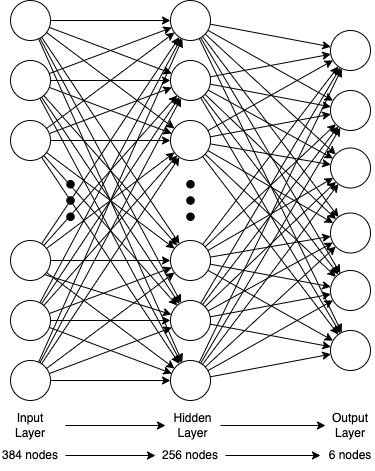
\includegraphics{eec_architecture.png}
	\caption{EEC Model Architecture}
	\label{fig:eec_architecture}
\end{figure}
\end{textblock}

\begin{textblock}{10}(11.5, 19.5)
\CHead{Model Performance}
The EEC model achieved a macro F1-score of 0.57 on the validation dataset. It was able to adequately identify happiness, sadness, and fear, but struggled with the other emotions. Disgust was regularly misclassified, and there remained confusion between surprise and happiness. This variance was expected due to the imbalanced training dataset. \\
\renewcommand{\thetable}{2}
\begin{table}[h]
    	\centering
    	\begin{tabular}{c c c c}
        		\toprule
        		\textbf{Emotion} & \textbf{Precision} & \textbf{Recall} & \textbf{F1-Score} \\
        		\midrule
        		Happiness & 0.75 & 0.76 & 0.76 \\
        		Sadness & 0.58 & 0.77 & 0.66 \\
        		Anger & 0.61 & 0.46 & 0.53 \\
        		Fear & 0.66 & 0.62 & 0.64 \\
        		Disgust & 0.49 & 0.32 & 0.39 \\
        		Surprise & 0.57 & 0.36 & 0.44 \\
        		\bottomrule
    	\end{tabular}
    	\caption{EEC Model Performance Statistics}
	\label{tab:eec_summary_statistics}
\end{table}
\end{textblock}

% Column 3
\begin{textblock}{10}(22.5, 04)
\CHead{Classifying Reviews}
The EEC model was used to classify the emotions expressed in the movie review dataset, a collection of 65,967 reviews gathered from top-rated movies on Letterboxd. As expected, happiness was the most common emotion, expressed in nearly 37\% of all reviews. The least frequent emotions were disgust and anger, combining for less than 8\%. \\
\renewcommand{\thetable}{3}
\begin{table}[h]
    	\centering
    	\begin{tabular}{c c c}
        		\toprule
        		\textbf{Emotion} & \textbf{Count} & \textbf{Percentage} \\
        		\midrule
        		Happiness & 24,404 & 36.99\% \\
        		Sadness & 17,924 & 27.17\% \\
        		Anger & 4,261 & 6.46\% \\
        		Fear & 12,754 & 19.33\% \\
        		Disgust & 633 & 0.96\% \\
        		Surprise & 5,991 & 9.08\% \\
        		\bottomrule
    	\end{tabular}
    	\caption{Distribution of Emotions in Movie Reviews}
	\label{tab:movie_review_distribution}
\end{table}
\end{textblock}

\begin{textblock}{10}(22.5, 11.5)
\CHead{Emotion Patterns}
Beyond the raw counts, the emotions expressed in reviews were stratified across different categories to identify less obvious patterns. First, the distribution of emotions expressed in reviews was found to be approximately the same regardless of the decade in which the movie was released. \\
\renewcommand{\thefigure}{2}
\begin{figure}[h]
	\centering
	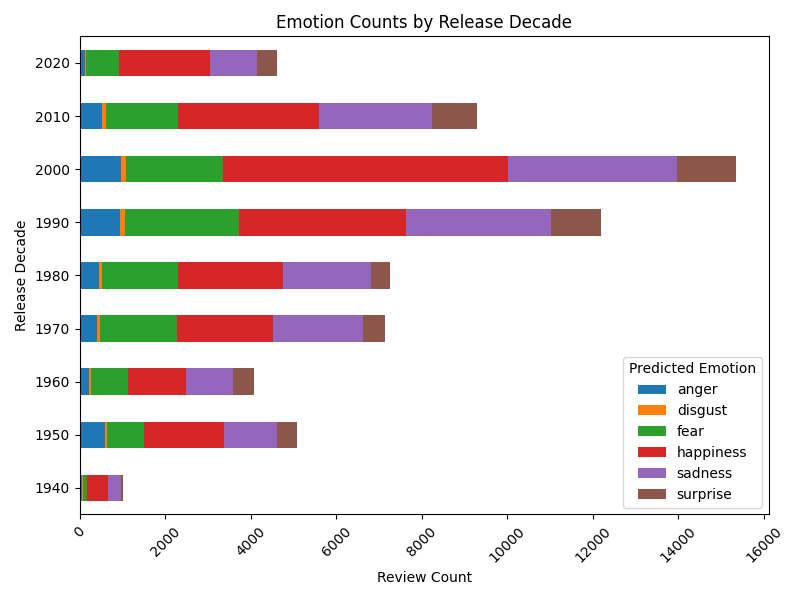
\includegraphics[width=0.75\textwidth]{emotion_counts_by_release_decade.png}
	\caption{Emotion Counts by Release Decade}
	\label{fig:emotion_counts_by_release_decade}
\end{figure}
Next, it was observed that the distribution of emotions expressed in reviews remained nearly identical to the overall distribution regardless of the movie's country of origin. \\
\renewcommand{\thefigure}{3}
\begin{figure}[h]
	\centering
	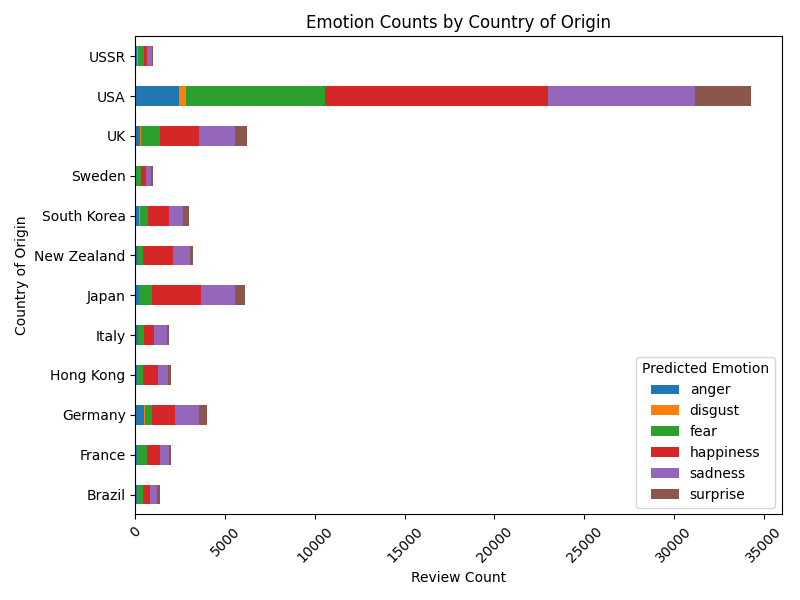
\includegraphics[width=0.75\textwidth]{emotion_counts_by_country.png}
	\caption{Emotion Counts by Country of Origin}
	\label{fig:emotion_counts_by_country}
\end{figure}
\end{textblock}

% Column 4
\begin{textblock}{10}(34, 04)
\CHead{More Emotion Patterns}
The most prevalent emotion in horror movie reviews was fear, and the most common emotion in history movie reviews was sadness. Meanwhile, a relatively high percentage of reviews for both thriller and mystery movies expressed surprise. \\
\renewcommand{\thefigure}{4}
\begin{figure}[h]
	\centering
	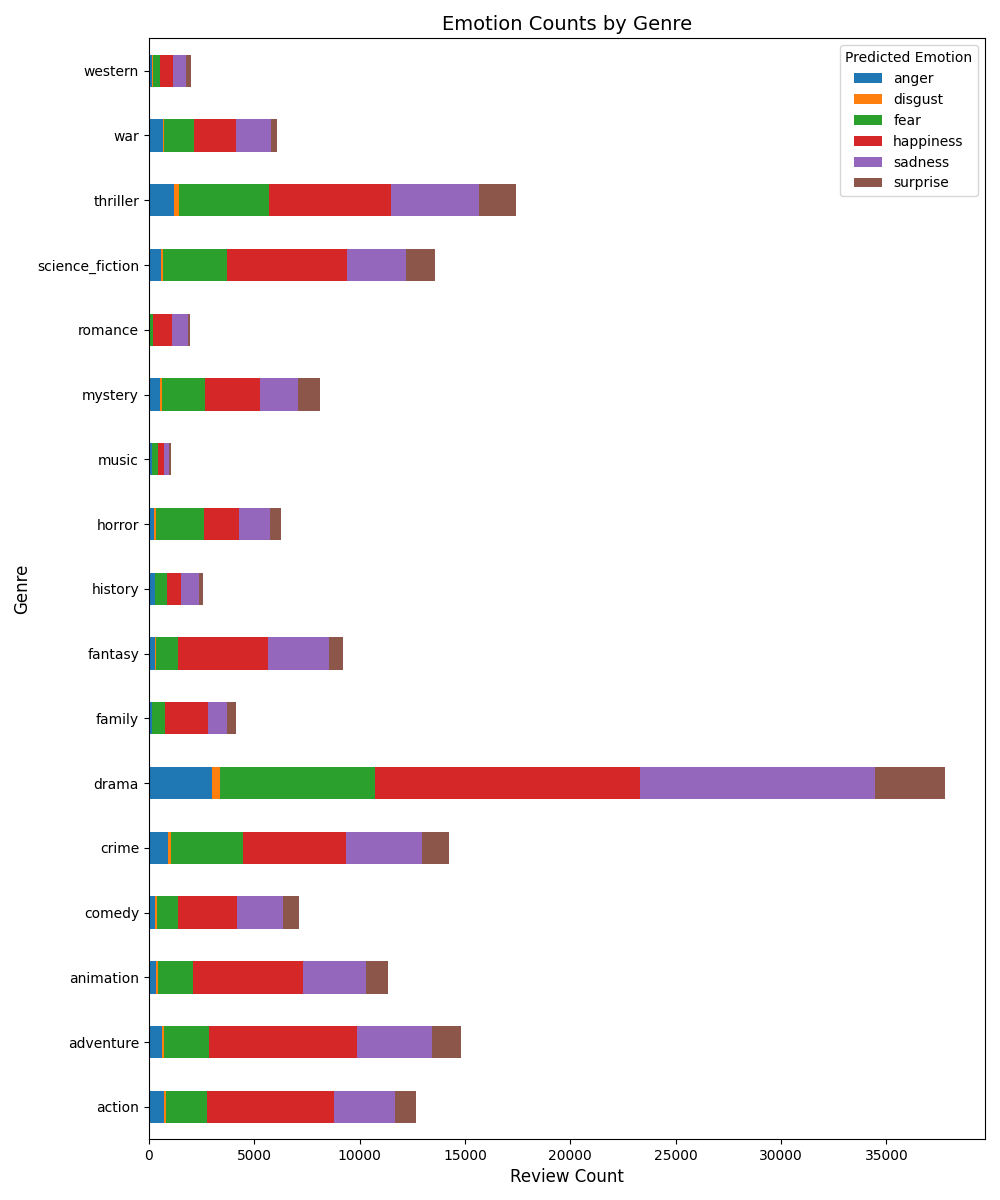
\includegraphics[width=0.75\textwidth]{emotion_counts_by_genre.png}
	\caption{Emotion Counts by Genre}
	\label{fig:emotion_counts_by_genre}
\end{figure}
On Letterboxd, users are also able to like reviews. Surprisingly, the reviews expressing the least frequent emotions received the most likes on average, and vice versa. \\
\renewcommand{\thefigure}{5.5}
\begin{figure}[h]
	\centering
	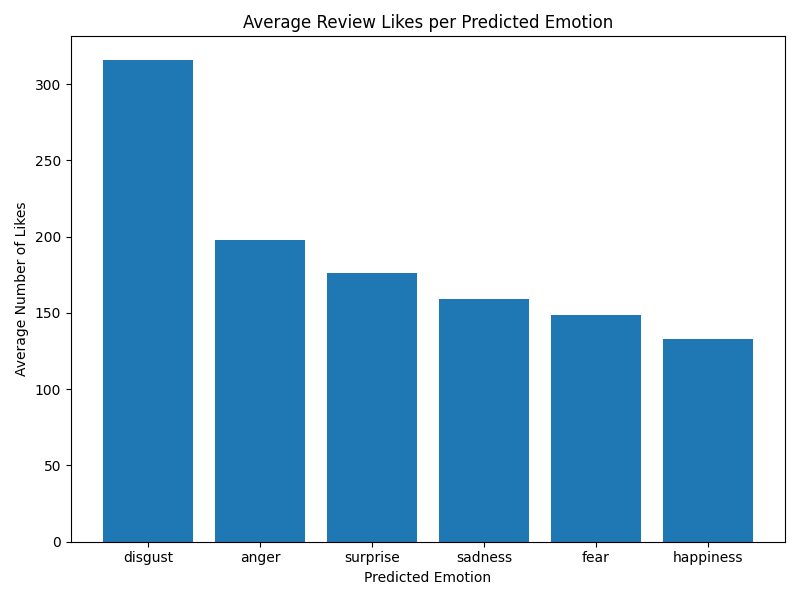
\includegraphics[width=0.75\textwidth]{average_likes_per_emotion.png}
	\caption{Average Review Likes per Emotion}
	\label{fig:average_likes_per_emotion}
\end{figure}
\end{textblock}

\begin{textblock}{10}(34, 22)
\CHead{Conclusion}
Our analysis revealed that happiness and sadness were the most frequently expressed emotions in reviews, but rarer emotions like disgust and anger tended to receive more likes on average. Surprisingly, the distribution of emotions expressed in reviews remained similar for movies released in different decades or originating from different countries. As expected, that the distribution of emotions varied across genres. Future work could verify these results using a better emotion classification model and further generalize the patterns by analyzing a larger dataset of movie reviews.
\end{textblock}

\end{document}